%==============================================================================
% Section 1: Introduction
%==============================================================================
\section{Introduction}
\label{sec:intro}

\subsection{Background and motivation}
\label{sec:intro:background}

The DPPU series has progressively organised the Einstein--Cartan plus
Nieh--Yan setting~\cite{Hehl1976,NiehYan1982} in terms of homogeneous
geometries, torsion modes, Pontryagin-type diagnostics, and topology
response~\cite{paper1,paper2,paper3,paper3ec,paper4}.  Paper~V~\cite{paper5}
constructed the $\alpha=0$ EC+NY baseline in Lorentzian signature on the
$\Sthree$ closed-FLRW branch, and established the channel separation among the
Hamiltonian constraint, the torsion auxiliary sector, and the diagnostic
quantities $\Pform$, $\Pint$, and $\QNY$.

The aim of the present paper is to extend that baseline to the four
topologies
\begin{equation}
  \Sthree, \quad \Tthree, \quad \Nilthree, \quad \Solthree,
\end{equation}
and to make explicit how topology dependence appears in the branch
classification and in the diagnostic structure.  The subject of this paper
is not bounce cosmology model building, but a classificatory analysis of
$\chi$-controlled topology universality in the reduced sector.

\subsection{Main results}
\label{sec:intro:results}

The main results of this paper are the following.

\begin{enumerate}
  \item In the Lorentzian EC+NY reduced setting, the four topologies
        $\Sthree$, $\Tthree$, $\Nilthree$, and $\Solthree$ share the same
        local admissibility pattern: $\EH$, $\AX$, and $\VT$ are admissible,
        while $\MX$ is conditionally admissible.

  \item On the active torsion branches, $\Pform$ vanishes exactly by block
        orthogonality.

  \item $\PintMX$ has a topology-universal functional template; the
        topology dependence is localised in the single coefficient
        $\Ctop = -9\chi$.

  \item $\QNY$ is an endpoint or boundary channel: zero on $\VT$,
        on-shell trivial on $\AX$, and boundary-conditional on $\MX$.

  \item On the auxiliary shell, the reduced vacuum orbit is governed by
        $\dot q^{2}+\chi=0$.

  \item Within this vacuum reduced atlas, no bounce-like or
        recollapse-like orbit class is found.
\end{enumerate}

The scalar $\chi$ in result~3 and in result~5 is obtained from independent
routes -- a symbolic analysis of $\PintMX$ and a derivation from the
$\EH$-spatial-curvature sector, respectively -- and the agreement of these
two routes is the substance of $\chi$-universality.

In other words, in the Lorentzian EC+NY reduced sector topology does not
alter the algebraic admissibility pattern, but controls the MX internal
diagnostic and the vacuum auxiliary-shell orbit through the same scalar
$\chi$.

\begin{figure}[H]
  \centering
  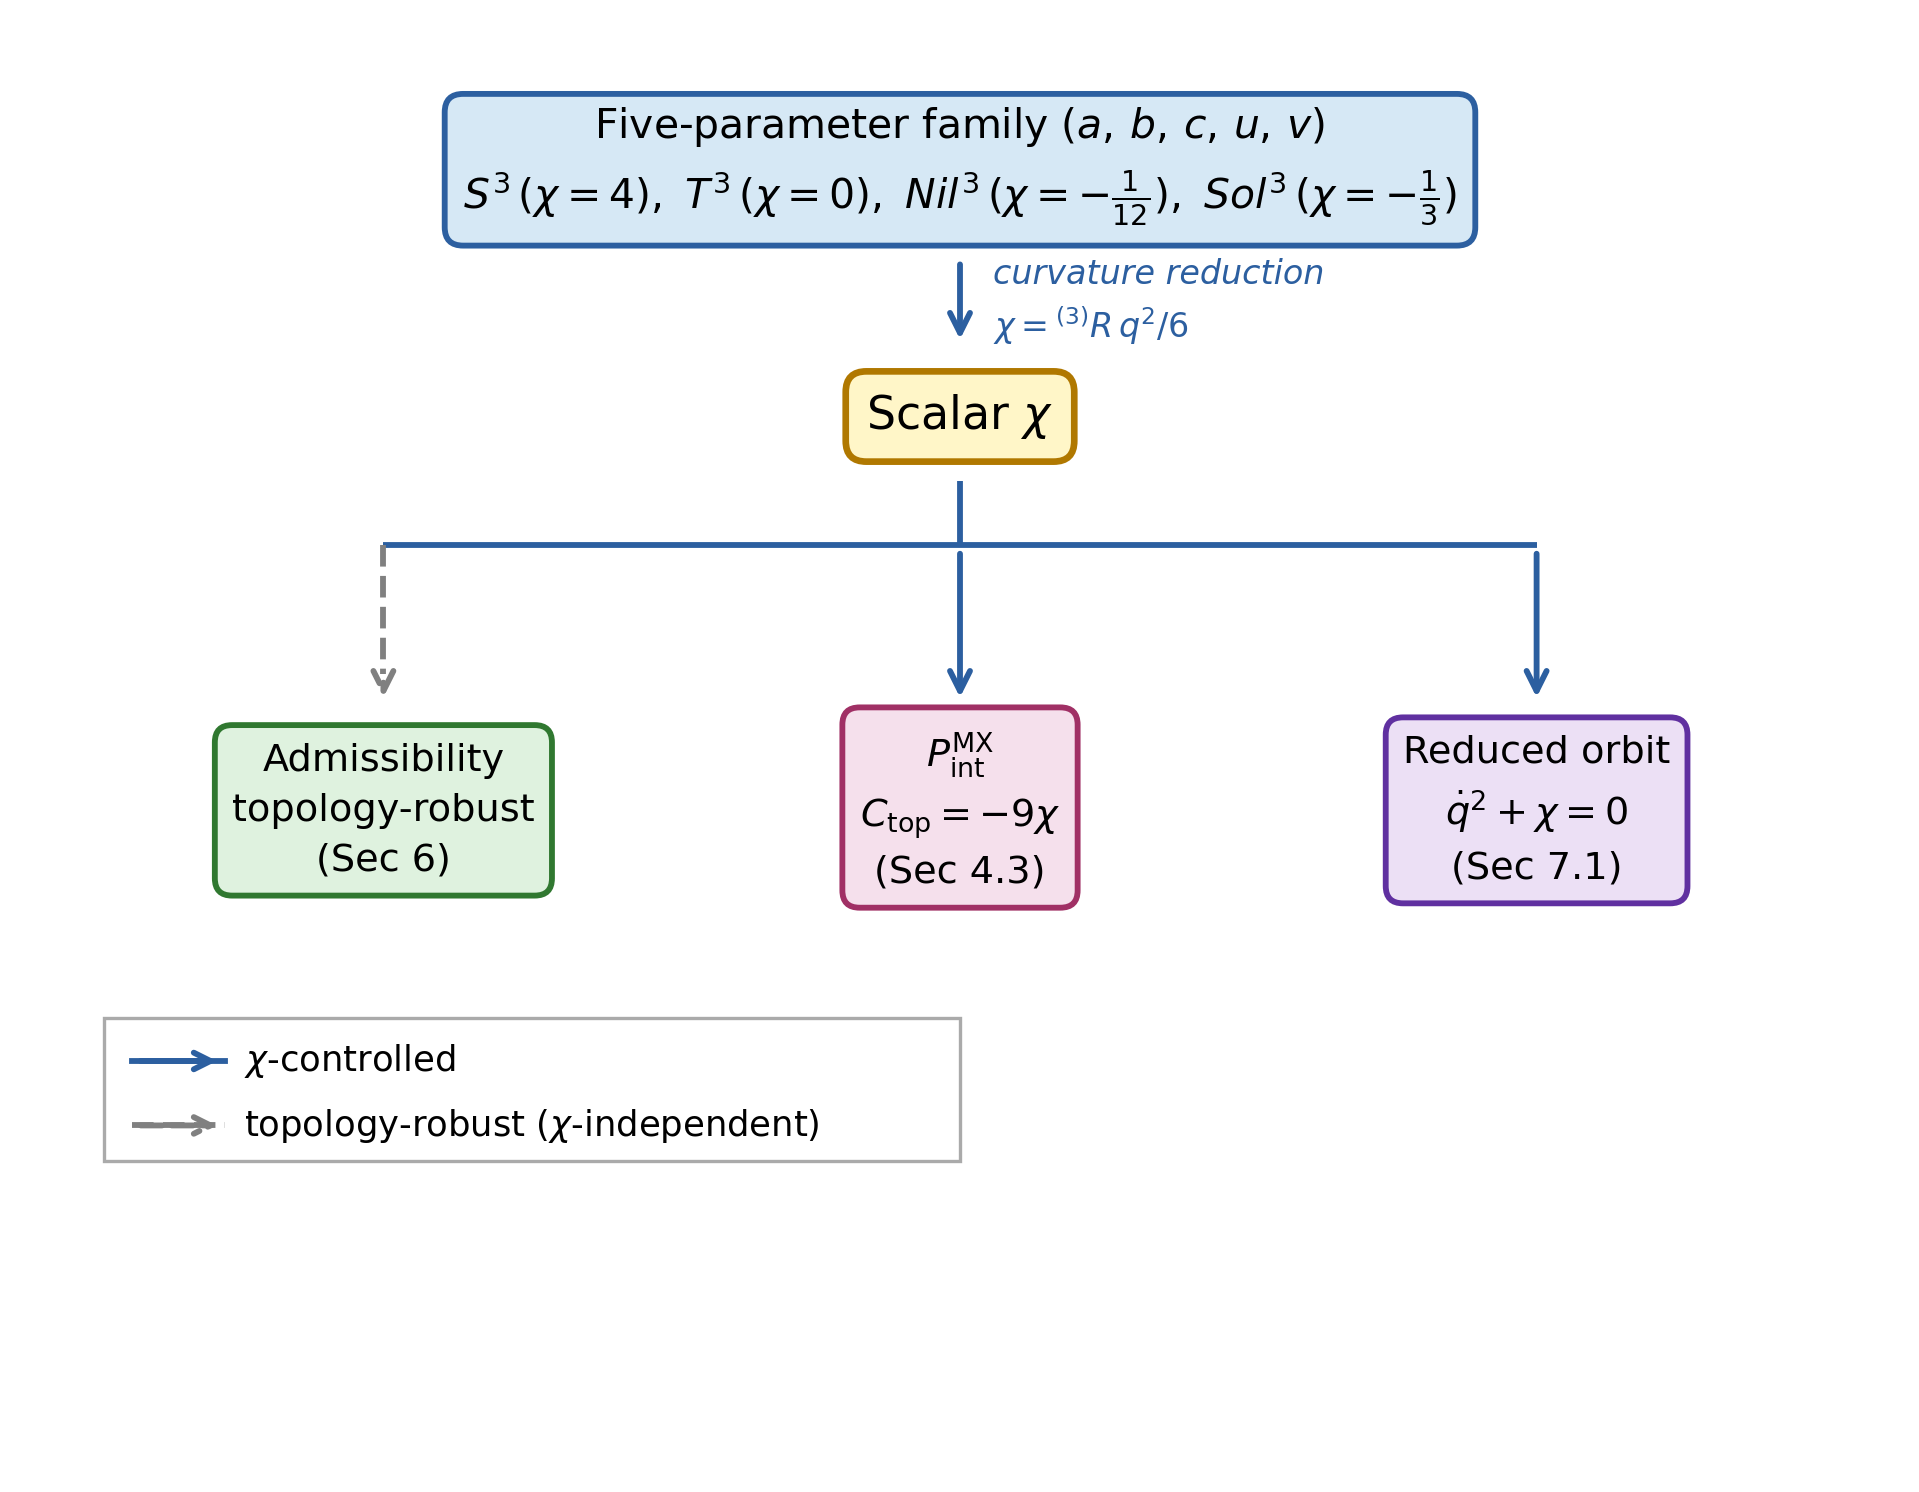
\includegraphics[width=0.9\textwidth]{figures/fig01_three_level_architecture.png}
  \caption{Three-level architecture of $\chi$-controlled topology
    universality in the reduced LZ-native isotropic EC+NY sector.  The
    five-parameter family $(a,b,c,u,v)$ at the top reduces, via the
    spatial-curvature contraction, to the scalar $\chi$, from which three
    independent consequences follow: the topology-robust admissibility
    pattern, the MX diagnostic identity $\Ctop=-9\chi$, and the reduced
    vacuum orbit $\dot q^{2}+\chi=0$.  The arrow to admissibility (dashed)
    indicates that the admissibility pattern does not depend on $\chi$.
    The arrows to $\PintMX$ and to the reduced orbit (solid) indicate
    $\chi$-mediated control.  \emph{Scope}: limited to the reduced
    LZ-native isotropic EC+NY sector; global, anisotropic, and
    matter-coupled extensions lie outside the scope of this paper.}
  \label{fig:three_level_architecture}
\end{figure}

\subsection{Relation to earlier DPPU papers}
\label{sec:intro:relation}

Paper~V~\cite{paper5} constructed the Lorentzian $\alpha=0$ EC+NY baseline on
$\Sthree$ and separated $\Pform$ from $\Pint$.  The present paper extends
that baseline to a four-topology table.

In particular, the $\Sthree$ row of the present paper reproduces the
$\alpha=0$ Lorentzian baseline of paper~V.  In Table~B1, the $\Sthree$ entry
has $F_{\mathrm{shell}}=4$, the $\MX$ auxiliary Hessian
$-4q^{2}(\kap^{4}\thetaNY^{2}+1)/9$, and the classification label
\code{L_CONDITIONALLY_ADMISSIBLE}.  The new content of the present paper is
that the same pattern extends to $\Tthree$, $\Nilthree$, and $\Solthree$.

In paper~IV~\cite{paper4} the same four Thurston
geometries~\cite{Thurston1997,Scott1983} produced four response types -- none,
uniaxial, triaxial, and biaxial -- in the Euclidean response dictionary.  As
discussed in Section~\ref{sec:bridge:loci}, the same four geometries reappear
here as structurally distinguished loci in the LZ-native isotropic
five-parameter family.  This correspondence is a structural resonance, and
its interpretation is taken up in Section~\ref{sec:discussion:paper04echo}.

\subsection{Organisation of the paper}
\label{sec:intro:outline}

Section~\ref{sec:setup} fixes the Lorentzian-native setup and the topology
conventions.
Section~\ref{sec:hamiltonian} states the Hamiltonian admissibility backbone.
Section~\ref{sec:pchannel} organises the channel dictionary for $\Pform$,
$\Pint$, and $\QNY$.
Section~\ref{sec:bridge} connects the diagnostic-level and reduced-orbit-level
$\chi$-universality.
Section~\ref{sec:classification} summarises the four-topology admissibility
classification.
Section~\ref{sec:orbit} states the reduced orbit atlas and the
$\chi$-sign separation.
Section~\ref{sec:discussion} discusses the meaning of $\chi$-universality,
the relation to paper~IV, and future directions.
Appendix~\ref{app:A} supplements the topology conventions, local reductions,
and caveats.
Appendix~\ref{app:B} collects tables, computational checks, and
reproducibility notes.
Appendix~\ref{app:C} states a Bianchi~I lite comparison and the reduced-atlas
scope guard.
